\documentclass{article}
\usepackage{graphicx}
\usepackage{float}
\usepackage{subfigure} 
\usepackage{amsmath}
\usepackage{amssymb}
\usepackage{listings}
\usepackage{color}
\usepackage{seqsplit}
\usepackage{geometry}
\geometry{left=0.5cm} 
\geometry{right=0.5cm}
\geometry{top=0.5cm}
\geometry{bottom=0.5cm}

\begin{document}
\section{The rules of game}
PAPI: Players, Actions, Payoffs, Information
Dominant Strategy: A strategy is dominant if it is the best strategy for A regardless of what B does.
Dominated Strategy: A strategy is dominated if there is another strategy that always gives a higher payoff.
For player i, strategy si is weakly dominated if there exists some other strategy s
i' which is possibly better and never worse, yielding a higher payoff
in some strategy profile and never yielding a lower payoff.\\
Nash Equilibrium: The strategy profile s* is a Nash equilibrium if no player has incentive to deviate from his strategy given that the other players do not deviate.\\
Perfect: Each information set is a singleton.  
Symmetric: No player has information different from
other players when he moves, or at the end
nodes. 
Asymmetric: Someone has private information . 
Complete: Nature does not move first, or her initial
move is observed by every player. \\
Harsanyi Transformation: Harsanyi suggests that to deal with a game with unclear rules, we can
transform the game by adding an initial move in which Nature chooses
between different sets of rules. In the transformed game, all players know the new meta-rules, including the
fact that Nature has made an initial move unobserved by them.
A state of the world is a move by Nature.\\
Harsanyi Doctrine: Different beliefs is modelled as the effect of observing different moves by
Nature. Players start with the same probabilities of Nature moves.\\
Herding Effect: One Bayesian Equilibrium looks like this:
Player 1: If sees signal high, accept; if sees signal low, reject.
Player 2: imitates player 1’s action, regardless of the value of his signal.
Player 3: imitates 1 and 2’s action, regardless of the value of his signal.\\
The welfare game:\\
\begin{figure}[H]
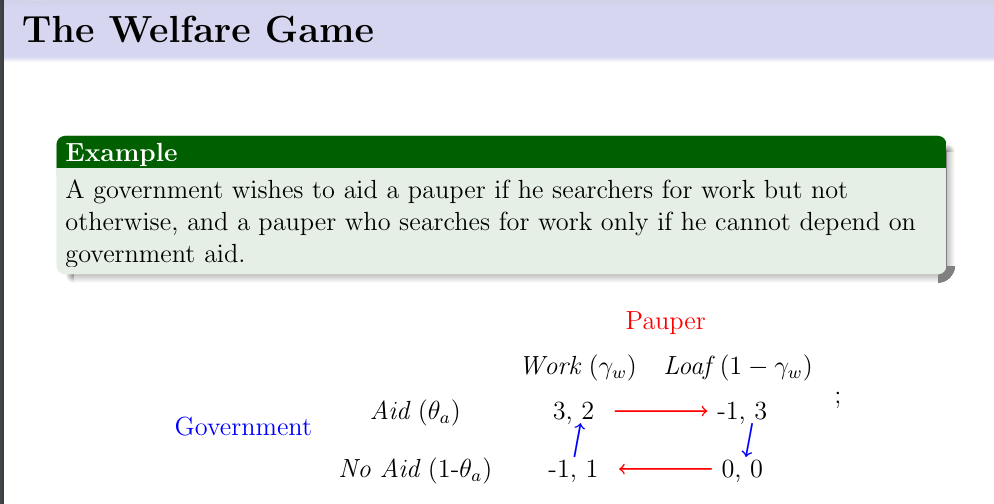
\includegraphics[width=0.3\textwidth]{welfare1.png}
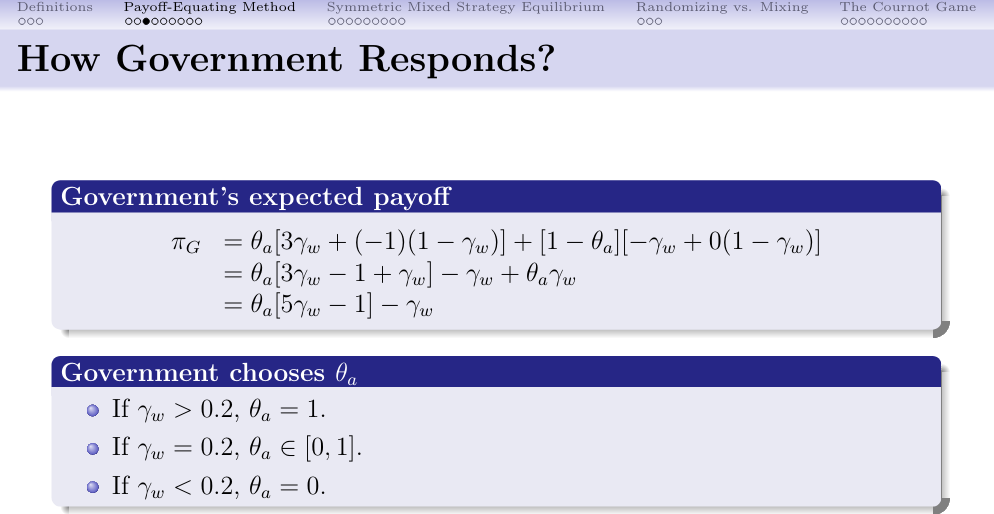
\includegraphics[width=0.3\textwidth]{welfare2.png}
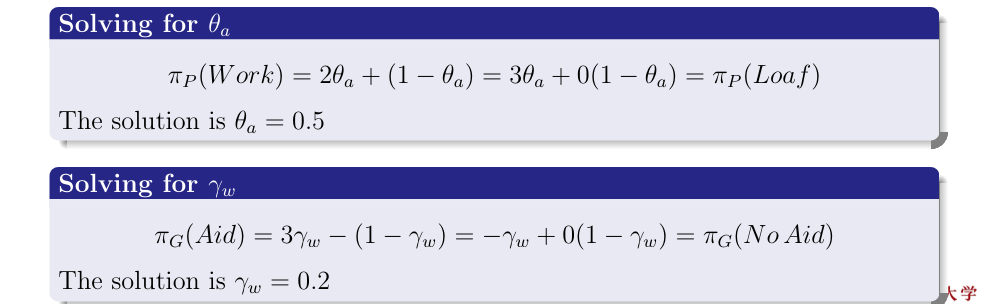
\includegraphics[width=0.3\textwidth]{welfare3.png}
\end{figure}
In the mixed strategy equilibrium, Government must be indifferent between
Aid and No Aid and Pauper must be indifferent between Work and Loaf.\\
War of Attrition:\\
\begin{figure}[H]
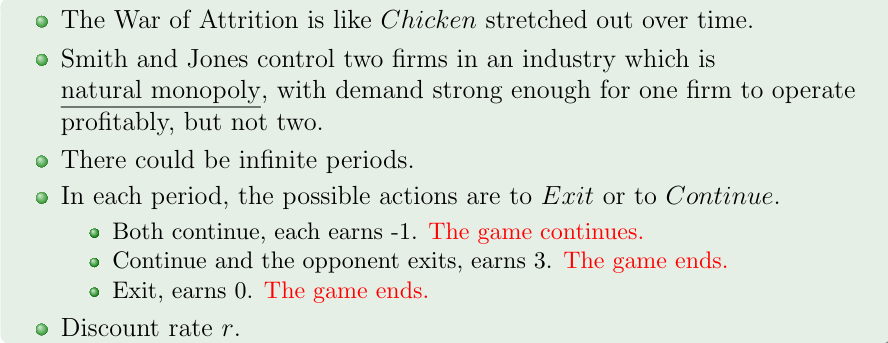
\includegraphics[width=0.4\textwidth]{attrition.png}
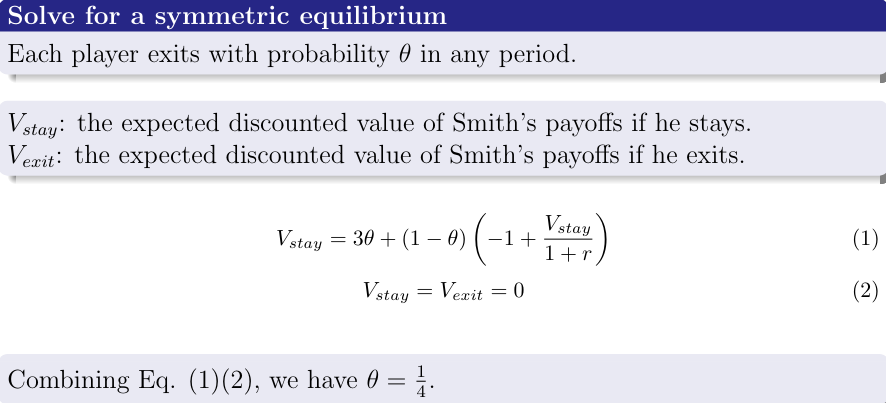
\includegraphics[width=0.4\textwidth]{attrition2.png}
\end{figure}
Patent Game: The cumulative distribution function for N-players game is $M(x) = (x/V)^{1/(N-1)}$\\
The Cournot Game:\\
\begin{figure}[H]
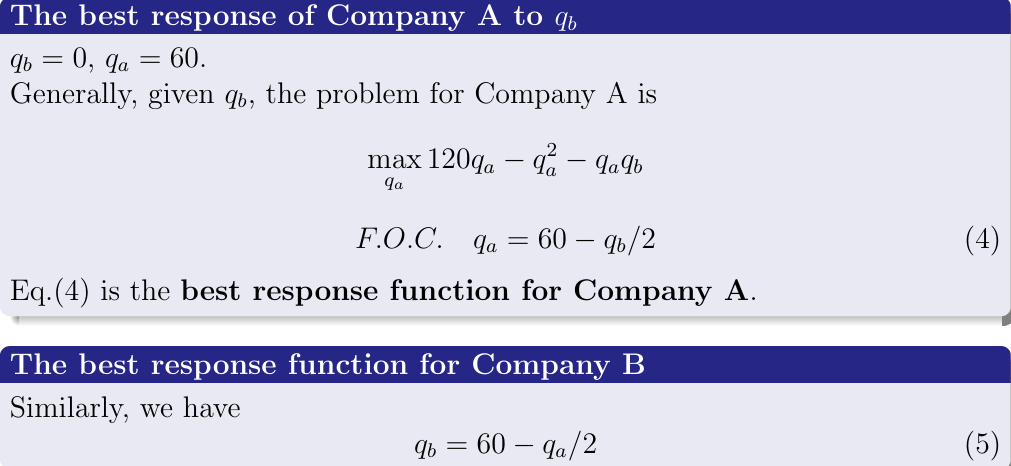
\includegraphics[width=0.33\textwidth]{cournot.png}
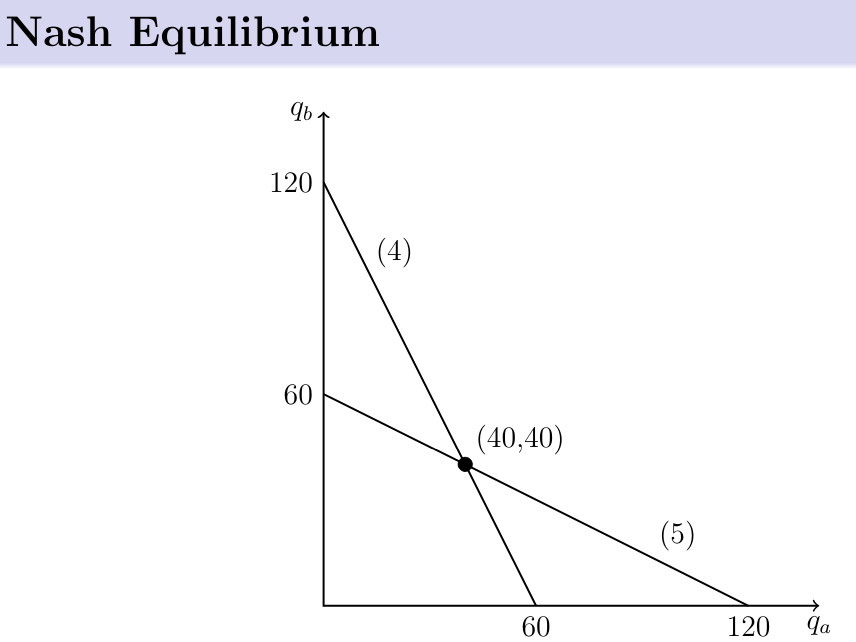
\includegraphics[width=0.33\textwidth]{cournot2.png}
\end{figure}
Equilibrium Path: is the path through the game tree that is followed in equilibrium. If a player deviates from the equilibrium strategy,
we say it is off the equilibrium path.\\
A subgame is a game consisting of a node which is a singleton in every
player’s information partition, that node’s successors, and the payoffs at the
associated end nodes.\\
A strategy profile is a subgame perfect equilibrium (SPE) if (a) it is a
Nash equilibrium for the entire game; and (b) its relevant action rules are a
Nash equilibrium for every subgame.
The small probability of a mistake is called a tremble. The trembling
hand approach is featured by allowing players to make mistakes with small
probabilities and examining whether a Nash equilibrium is robust to this
change in the game.\\
Chainstore Paradox: SPE: Grim Strategy(Start by choosing Deny. If the other player ever chooses Confess, then choose Confess forever after.) Tit-for-Tat(Start by Start by choosing Deny. In period n, choose the action that the other player chose in period (n - 1)) Tit-for-Tat is not an equilibrium strategy\\
Minimax Strategy and the Folk Theorem(Note that the crossing part is the The set of SPE payoff profiles)\\
\begin{figure}[H]
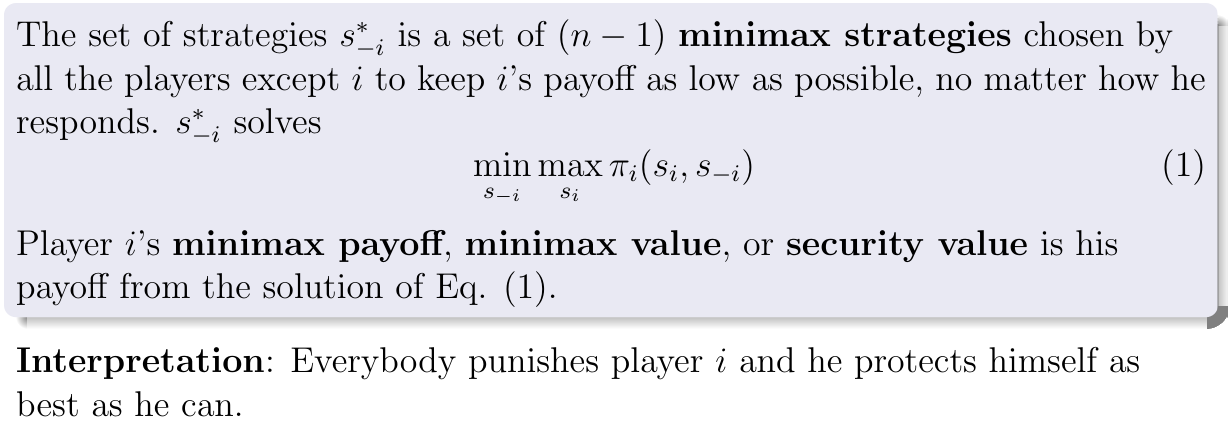
\includegraphics[width=0.33\textwidth]{minmax.png}
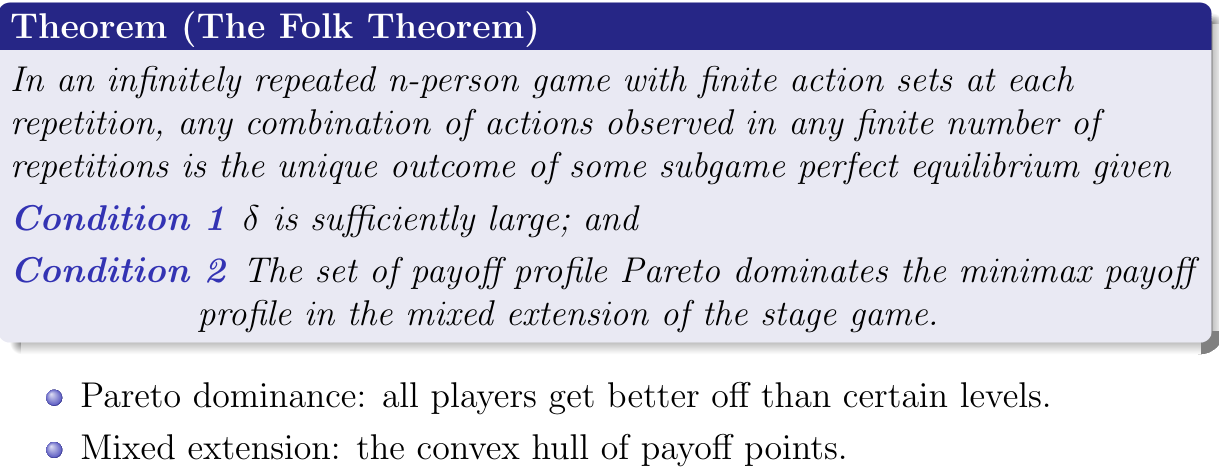
\includegraphics[width=0.33\textwidth]{Folk.png}
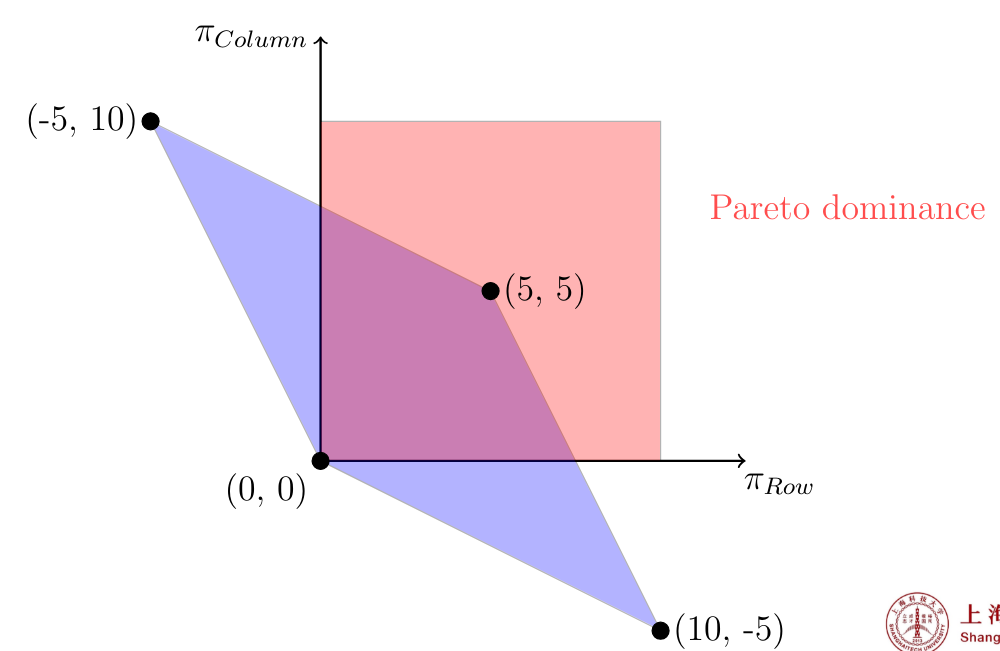
\includegraphics[width=0.33\textwidth]{pd.png}
\end{figure}
Perfect Bayesian Equilibrium: Separating Equilibrium(Can update beliefs) and Pooling Equilibrium(No update beliefs). When the equilibrium is out of the path, you need to somehow choose your beliefs, whether it is passive conjecture or others.\\
\begin{figure}[H]
    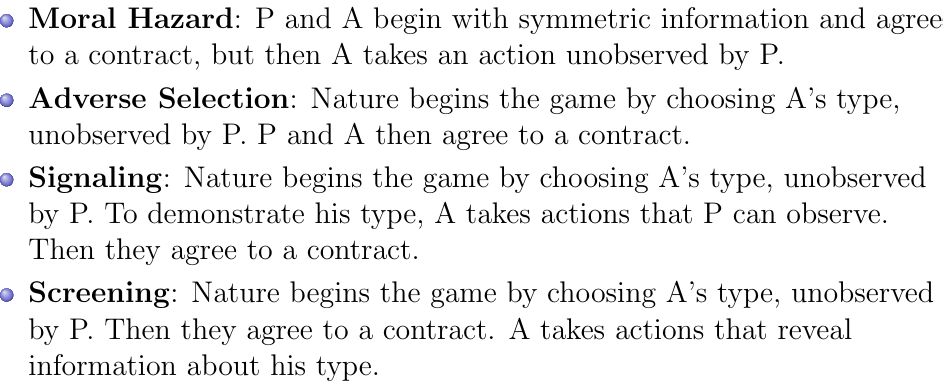
\includegraphics[width=0.33\textwidth]{moral.png}
    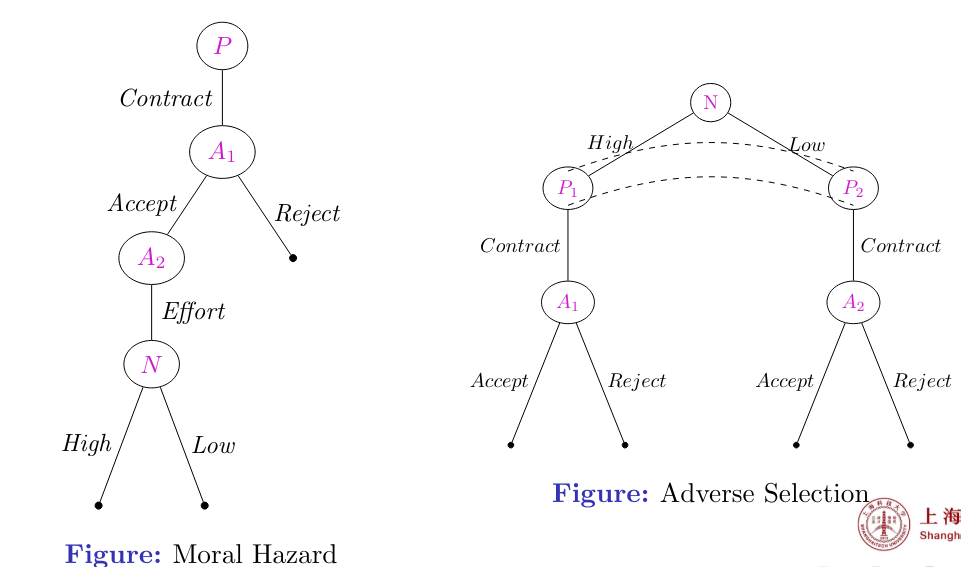
\includegraphics[width=0.33\textwidth]{moral2.png}
    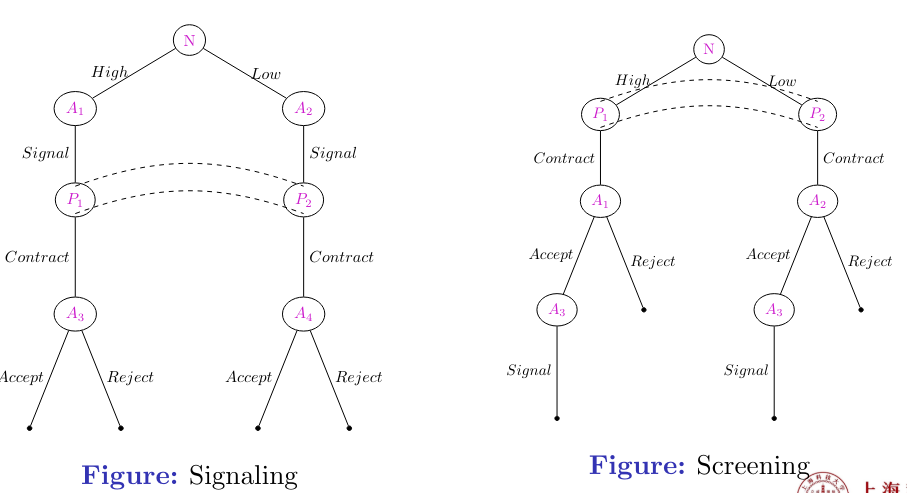
\includegraphics[width=0.33\textwidth]{moral3.png}
\end{figure}
\begin{figure}[H]
    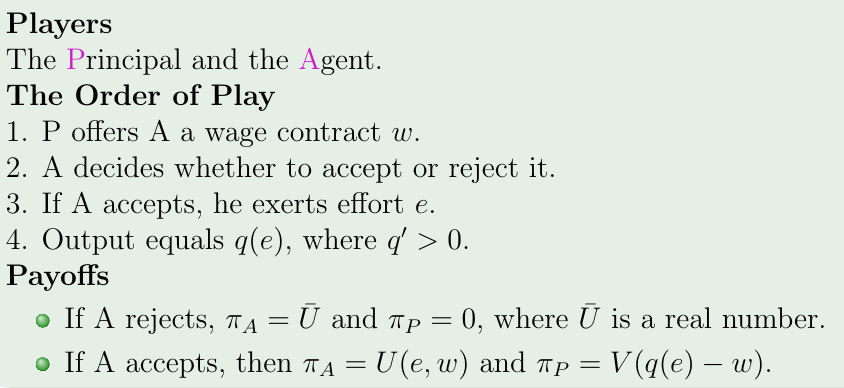
\includegraphics[width=0.33\textwidth]{production2.png}
    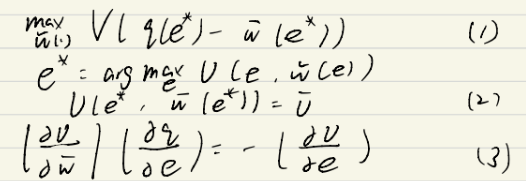
\includegraphics[width=0.33\textwidth]{production.png}
    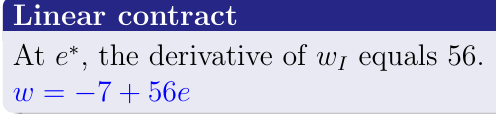
\includegraphics[width=0.33\textwidth]{production3.png}
\end{figure}
Production Game: Incentive compatibility: the payoff to be honest is no less than the payoff to be embezzle. Participation: the payoff to be honest is higher than Reservation utility\\ 
\begin{figure}[H]
    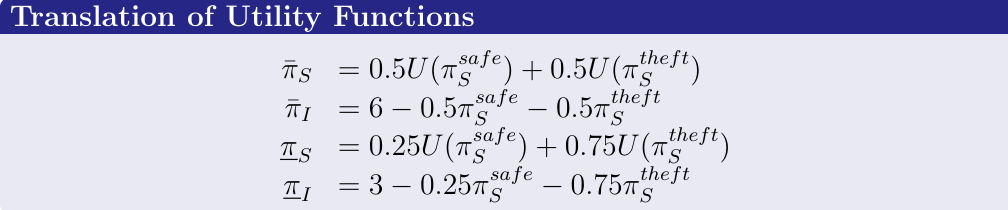
\includegraphics[width=0.3\textwidth]{insurance.png}
    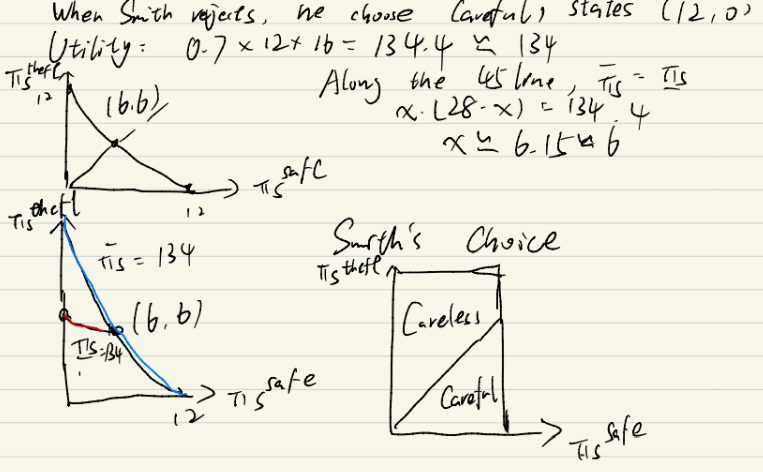
\includegraphics[width=0.3\textwidth]{insurance2.png}
    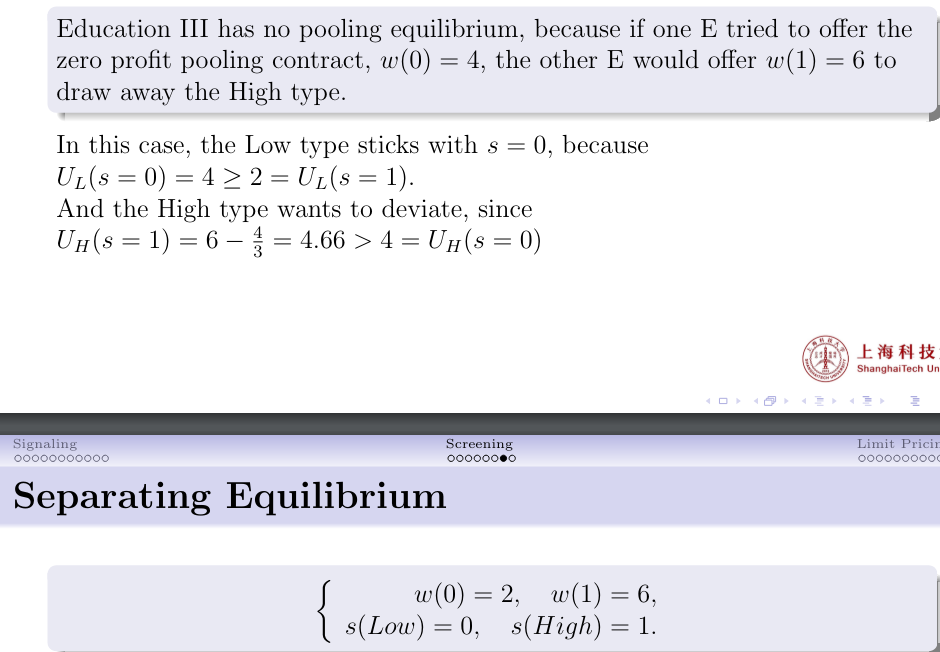
\includegraphics[width=0.3\textwidth]{signal.png}
\end{figure}
Signaling: Separating Equilibrium and Pooling Equilibrium are all under participation and incentive compatibility.\\
\end{document}